\documentclass[12pt]{article}

\usepackage{sbc-template}
\usepackage{graphicx,url}
\usepackage[utf8]{inputenc}
\usepackage[brazil]{babel}
\usepackage[latin1]{inputenc} 
     
\sloppy

\title{Aplicação de Sistema Embarcado Linux em Chatbot Acadêmico}

\begin{document} 

\maketitle

\begin{abstract}
It is often observed barriers of communication and transmission of information on higher education institutions. Conversational agents aimed at meeting the students can be used to overcome these problems, but there are still many universities that have not joined the technology. In this study are addressed the challenges faced by students of the educational institution and is presented "Kinho", a chatbot that guides users on the operation of academic space. “Kinho” was developed to run on an embedded system based on the Raspberry Pi. The chatbot uses the concepts of NLP to carry out the understanding process of the questions and then respond accordingly to the user. Experiments testing the system showed great acceptance of the solution by the internal academic community.
\end{abstract}
     
\begin{resumo} 
Frequentemente é observado barreiras de comunicação e transmissão de informações nas instituições de ensino superior. Agentes conversacionais voltados ao atendimento aos alunos podem ser utilizados para superar esses problemas, mas ainda existem muitas universidades que não aderiram à tecnologia. Neste estudo são abordados os desafios enfrentados pelos estudantes da instituição de ensino e é apresentado “Kinho”, um chatbot que orienta os usuários sobre o funcionamento do espaço acadêmico. “Kinho” foi desenvolvido para ser executado em um sistema embarcado baseado no Raspberry Pi. O chatbot utiliza dos conceitos de NLP para realizar  o processo de entendimento das perguntas e então responder adequadamente ao usuário. Experimentos de testes com o sistema mostraram uma grande aceitação da solução por parte da comunidade acadêmica interna.
\end{resumo}


\section{Introdução}

A cada novo semestre, alunos novatos ingressam em uma instituição de ensino superior e encontram um ambiente educacional com estruturas diferentes do que estão acostumados. De acordo com \cite{torres:21} houve uma diversificação social na população que passou a frequentar a universidade, em que é observado o ingresso de estudantes de famílias de baixa renda, muitas vezes os primeiros de sua família a frequentar a universidade. Esses estudantes encontram um período de adaptação ao ensino superior muito mais significativo, pois vários deles ingressam sem as competências ou recursos necessários para frequentar a universidade, assim como não costumam compartilhar da cultura dos membros da instituição. 

É muito comum que estudantes sintam-se desinformados sobre o funcionamento do novo ambiente e busquem orientações de terceiros. Geralmente são os estudantes de classes sociais menos favorecidas que mais necessitam de acolhimento institucional e psicopedagógico por parte dos professores e colegas, mas são os que mais carecem dessa atenção especial para se aproximar da nova realidade do ensino superior \cite{torres:21}.

Com base em um levantamento interno realizado pelos autores através da aplicação de um questionário utilizando o serviço de formulários do {\itshape Google}, foi observado que muitos alunos recorrem a grupos de aplicativos de {\itshape chat} para obter informações não oficiais, muitas vezes desobedecendo regras gerais do grupo ou até mesmo não conseguindo ingressar por conta de um limite máximo de usuários ou não obtenção do {\itshape link} de acesso. Além disso, as perguntas dos estudantes costumam ser repetitivas e possuem um certo padrão, o que permite buscar uma solução para automatizar o processo de atendimento.

{\itshape Chatbots} (do inglês {\itshape chat robots}, ou “robôs de conversação”) são agentes de conversação ou aplicativos inteligentes que simulam a conversação como se fossem seres humanos \cite{lucchesi:18}. {\itshape Chatbots} podem ser utilizados em empresas para auxiliar na comunicação, em trocas e devoluções de produtos e atendimento aos clientes \cite{correia:19} \cite{valente:20}, mas seu uso não se limita somente ao ramo empresarial.

Qualquer pessoa pode criar um {\itshape chatbot} para conversar, gerenciar informações e executar operações, realizar pesquisas de opinião, jogar ou até mesmo controlar dispositivos de Internet das Coisas (IoT, na sigla em inglês para {\itshape Internet of Things}). Entretanto, não é fácil incorporar sentimentos a eles, o que pode distanciá-los da humanização pretendida. Além disso, certos projetos exigem um elevado grau de conhecimento e é difícil encontrar especialistas na área, o que pode tornar a implementação de chatbots complicada e elevar custos \cite{guerreiro:19}.

Tendo em vista suas diversas aplicações e a problemática recorrente enfrentada pela instituição com relação à obtenção de informações pelos novos alunos, foi desenvolvido e testado um {\itshape chatbot} para o meio acadêmico com o intuito de responder algumas das dúvidas mais frequentes do corpo discente da instituição. A escolha da elaboração de um chatbot é baseada nos estudos de sistemas similares \cite{araujo:20} \cite{bulhoes:20} \cite{lucchesi:18} \cite{maciel:19} \cite{silva:21} em que foi observado uma boa resposta de estudantes e servidores no uso de {\itshape chatbots} voltados para o meio acadêmico, seja no campo educacional ou em orientações acerca do funcionamento da instituição de ensino.

A lógica de programação e interface gráfica do agente conversacional “Kinho” foram implementadas na linguagem Python, e o sistema foi embarcado em um Raspberry Pi (Rpi). A utilização de um sistema embarcado tem como objetivo reutilizar estruturas eletrônicas ociosas no campus ({\itshape totens}) que já estão equipadas com os monitores e teclados necessários para o funcionamento do sistema. No entanto, as novas restrições impostas pela instituição para impedir a disseminação do novo Coronavírus impediram que os testes práticos nos {\itshape totens} fossem executados.

Resultados experimentais demonstraram que o uso dessa aplicação diminuiu a dependência do estudante para recorrer a grupos de {\itshape chat} para obter informações repetitivas. Cerca de 82\% dos estudantes que participaram do teste afirmaram que utilizariam o chatbot para obter informações acadêmicas, 75\% afirmaram que o sistema facilita a comunicação do estudante com canais oficiais de comunicação e 89\% observaram a diminuição do tempo de resposta para tirar dúvidas relacionadas à instituição.


\section{ Fundamentação Teórica}

O uso de {\itshape chatbots} foi amplamente utilizado para diversos fins, seja empresarial, acadêmico ou pessoal. No que diz respeito aos trabalhos voltados à utilização no meio acadêmico, alguns projetos mostraram resultados positivos e boa aceitação do público, como é o caso do trabalho de \cite{silva:21}. O projeto apresenta um {\itshape chatbot} para auxiliar a comunidade do Instituto Federal de Brasília buscando informações no portal institucional para responder dúvidas dos estudantes relacionadas ao espaço acadêmico. O chatbot foi desenvolvido na linguagem Python para ser utilizado no aplicativo de mensagens {\itshape Telegram}. Segundo os autores, nas fases de teste com o protótipo observou-se que 11 dos 12 entrevistados conseguiram obter sucesso em suas pesquisas na primeira tentativa de uso do sistema.

Pode ser citado também o trabalho elaborado por \cite{maciel:19}. Em sua pesquisa, o autor realiza uma pesquisa entre diversas plataformas disponíveis para escolher aquela que melhor se adequa às especificidades do projeto e implementa “Maciel”, um {\itshape chatbot} para ser utilizado na Universidade Federal do Ceará (UFC) campus Russas oferecendo apoio ao corpo discente. O {\itshape chatbot} foi criado com a ferramenta {\itshape Dialogflow} e integrado ao aplicativo de mensagens {\itshape Whatsapp}, recebendo uma avaliação positiva entre os usuários e melhorias após os testes iniciais.

Outros {\itshape chatbots} acadêmicos são utilizados como ferramentas de apoio ao ensino, como é o caso do trabalho de \cite{bulhoes:20}, em que  foi desenvolvido um {\itshape chatbot} para auxiliar estudantes no processo de interpretação textual. O agente conversacional é implementado com uma interface gráfica em Java, realizando perguntas a partir de um texto que é exibido ao leitor. O programa faz uso de um interpretador para processar o texto digitado pelo usuário e consultar a melhor resposta na base de dados. Dentre os 50 alunos que utilizaram o programa, 48 afirmaram que as perguntas feitas pelo  {\itshape chatbot} contribuíram de forma relevante para o entendimento do texto.

Outro trabalho com resultados promissores é o de \cite{araujo:20}. O autor detalha o desenvolvimento de um {\itshape chatbot} para responder perguntas/dúvidas de alunos da disciplina de estrutura de dados, seguindo a ementa definida para a disciplina ministrada na UFC - Campus Russas. Apesar da maioria dos usuários declarar que o sistema apresenta dificuldades de uso, cerca de 76,8\% dos alunos  vêem benefícios na utilização de um {\itshape chatbot} para auxiliar suas atividades.

O projeto em  \cite{lucchesi:18} apresenta a criação do agente conversacional “Metis”, projetado para conversar com alunos como apoio às atividades de educação a distância. Foi realizado um estudo qualitativo acerca do funcionamento dos {\itshape chatbots} e seu potencial uso na educação. A análise dos resultados mostrou que houve um aumento, ainda que moderado, da média geral alcançada pelas turmas que utilizaram o agente para auxiliar seus estudos.

A Tabela 1 relaciona os trabalhos anteriormente analisados com suas principais características de desenvolvimento de {\itshape chatbots}. A utilização dos {\itshape chatbots} possuem objetivos "educacionais" quando são projetados para auxiliar os estudos dos estudantes em uma determinada disciplina, e "orientações" quando o objetivo é fornecer informações acerca do espaço acadêmico.

\begin{table}[h]
\caption{Trabalhos similares e principais características}
\label{table:1}
\begin{tabular}{ |p{3cm}|p{1.9cm}|p{2cm}|p{2.6cm}|p{3.4cm}|  }
 \hline
Autor & Plataforma & Utilização & Disponibilidade & Precisão das Respostas\\
 \hline
 \cite{araujo:20}   & {\itshape Web}    & Educacional &   Somente testes & 46,5\% das respostas são parcialmente corretas\\
  \hline
 \cite{bulhoes:20}&   {\itshape Desktop}  & Educacional   & Código aberto & 32\% das respostas são corretas
\\
 \hline
 \cite{silva:21} & {\itshape Mobile} & Orientações &  Somente testes & 96,7\% das respostas são corretas
\\
 \hline
 \cite{lucchesi:18}    & {\itshape Web} & Educacional & Código aberto & 82\% das respostas são parcialmente corretas \\
  \hline
 \cite{maciel:19}  & {\itshape Mobile}  & Orientações & Somente testes & Não avaliada
 \\
 \hline
\end{tabular}
\end{table}


A partir do estudo dos sistemas similares foi possível observar uma boa recepção dos usuários aos {\itshape chatbots}. A maioria dos sistemas não é de código aberto e possui uma eficiência parcial no que se diz respeito à obtenção de respostas no sistema. Somente o trabalho de \cite{silva:21} conseguiu uma precisão satisfatória, mas os testes foram realizados com questionamentos automatizados por botões, o que afeta a proposta de simulação de conversas humanizadas oferecidas pelos {\itshape chatbots}.

“Kinho” é um {\itshape chatbot} que oferece um sistema eficiente e humanizado para orientar os estudantes acerca do funcionamento da instituição de ensino superior, de código aberto e que explore as funcionalidades oferecidas pelo Raspberry Pi. O Raspberry Pi OS (anteriormente chamado Raspbian) é atualmente o sistema operacional oficial para todos os modelos de Raspberry Pi. Muitas aplicações e módulos dedicados à programação já vêm incluídos na imagem do Raspberry Pi OS, bastando iniciar o sistema para acessá-las \cite{juca:18}.

Projetos de sistemas embarcados em Raspberry apresentam resultados promissores, como é o caso do trabalho de \cite{junior:19}.  Os autores desenvolvem um sistema de confirmação de refeições do restaurante acadêmico do Instituto Federal de Educação, Ciência e Tecnologia do Ceará (IFCE), oferecendo uma alternativa ao método de confirmação existente. 

\section{Materiais e Métodos} \label{sec:firstpage}

O chatbot “Kinho” possui três componentes principais: base de dados, processamento das requisições e interface com o usuário, exibida na Figura 2 na seção Resultados e Discussões. Para construir a base de dados foi realizado um estudo sobre perguntas frequentes relacionadas a assuntos acadêmicos que estudantes realizavam no aplicativo de mensagens {\itshape Whatsapp} entre os meses de janeiro e agosto de 2021. As conversas de um grupo de avisos com cerca de 245 membros foi utilizado para construir a base de respostas padrões do {\itshape chatbot}.

Foi reunido um acervo abrangendo 200 perguntas e classificadas em 10 temas distintos. Para o tema “trancamento de disciplina”, por exemplo, observou-se duas perguntas mais frequentes entre os alunos: qual o período para realizar o procedimento e onde o estudante pode solicitá-lo. Dessa forma, foram elaboradas diversas sentenças que podem responder essas questões e registradas em um arquivo de texto. Esse documento é a base de dados a ser utilizada pela aplicação desenvolvida. A Tabela 2 relaciona algumas das perguntas, respostas mais adequadas e seus respectivos temas.

\begin{table}[h]
\caption{Perguntas e respostas do {\itshape chatbot}. O sistema encontra a melhor resposta relacionando as palavras-chave encontradas (destacadas em negrito) com as sentenças que contém essas palavras.}
\label{table:1}
\begin{tabular}{ |p{4.25cm}|p{5cm}|p{4.25cm}|  }
 \hline
Pergunta & Resposta do sistema & Tema\\
 \hline
 “Bom dia, você sabe as \textbf{datas} para o \textbf{reingresso}?”   & As \textbf{datas} para \textbf{reingresso} e reabertura de matrícula são entre os dias 01/03 e 04/03 &   Reingresso/Reabertura de Matrícula \\
 \hline
 “Qual o \textbf{link} pra \textbf{trancar} uma cadeira?”   & Para \textbf{trancar} uma disciplina, acesse o \textbf{link}: placeholder.link.com. &   Trancamento de Disciplina \\
 \hline
 “Tem alguma lista com \textbf{email} dos \textbf{professores}?”   & Para obter informações como \textbf{email} ou telefone dos \textbf{professores} de sua instituição, acesse: placeholder.link.com. &   Contatos dos Professores \\
 \hline
 “Onde podemos \textbf{conferir} se as \textbf{carteirinhas} já chegaram?”   & Você pode \textbf{conferir} a situação das \textbf{carteirinhas} no site: placeholder.link.com &   Carteira estudantil \\
 
 \hline
\end{tabular}
\end{table}

Para implementar o {\itshape chatbot} foi utilizada a biblioteca NLKT (do inglês {\itshape Natural Language Toolkit}, ou “Ferramentas de Linguagem Natural”) da linguagem Python. Essa biblioteca é um conjunto de recursos que realizam o processamento de linguagem natural (NLP, sigla em inglês para {\itshape “Natural Language Processing”}) para entender e simular a linguagem humana.

No momento em que o usuário envia sua pergunta ao sistema, as palavras passam pela “tokenização”: processo em que são separadas uma das outras pelas pontuações na sentença e pelos espaços em branco entre as palavras. Esse mesmo processo é feito nas respostas do {\itshape chatbot}. Após isso o programa realiza a “normalização”, que é um conjunto de procedimentos para remover letras maiúsculas e caracteres especiais das palavras. As palavras-chave são identificadas em ambos os textos analisando a frequência de menor ocorrência de cada uma, pois palavras mais raras são as que apresentam maior relevância para o sistema.

Se a sentença digitada pelo usuário contém palavras-chave que correspondem às respostas para os temas, o {\itshape chatbot} exibe a resposta mais adequada (a maior quantidade de palavras-chave iguais às digitadas pelo usuário). Caso contrário, o agente indica que não conseguiu entender a pergunta. Para maximizar as chances da pergunta do usuário ser entendida pelo programa, o ideal é que exista diversas sentenças de resposta para cada tema.

Antes da primeira interação do usuário com o {\itshape chatbot} é exibida uma mensagem de saudação indicando que as palavras “ajuda”, {\itshape “help”} ou “temas” podem ser digitadas a qualquer momento para exibir as áreas de conhecimento do programa. Dessa forma, é esperado que o usuário possa se orientar caso suas perguntas não sejam entendidas ou precise de orientação caso não saiba o que digitar. Além disso, foi implementado um histórico de conversa. As sentenças digitadas pelo usuário e suas respectivas respostas são registradas e exibidas para o usuário durante o funcionamento do programa simulando o funcionamento de aplicativos de mensagens conhecidos, como {\itshape Whatsapp} e {\itshape Telegram}.

A Figura 1 exibe a estrutura lógica de funcionamento do {\itshape chatbot} evidenciando os procedimentos utilizados para processar os textos e identificar a resposta adequada para a pergunta do usuário.

\begin{figure}[ht]
\centering
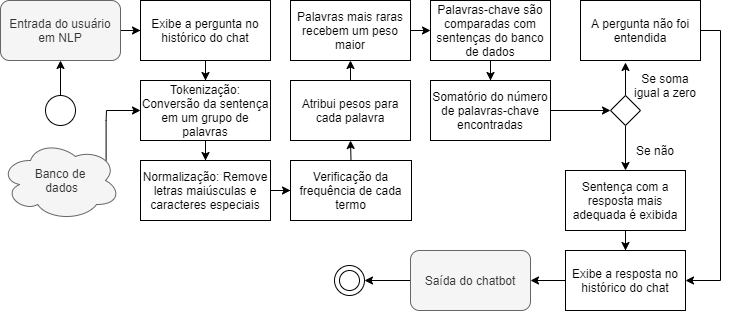
\includegraphics[width=1\textwidth]{fig1.png}
\caption{Fluxograma do processamento do {\itshape chatbot}. Após o usuário realizar uma pergunta, ela é processada por diversas etapas para que sua semântica seja capturada. Esse processo é chamado de “etapa de atenção” do {\itshape chatbot}. Se a pergunta for entendida pelo sistema, ele retornará uma resposta adequada em formato textual. }
\label{fig:exampleFig1}
\end{figure}

O {\itshape chatbot} foi executado em uma máquina virtual criada com o {\itshape software VirtualBox}. A máquina possui configurações mínimas de memória e armazenamento de disco, e foi configurada com um Raspberry Pi OS utilizando sistema operacional Debian 64 bits. O {\itshape chatbot} é executado com as versões 3.0 ou superiores do Python. Foi necessária a instalação adicional das bibliotecas NLTK, Numpy e Scikit-learn, assim como os pacotes “punkt” e “wordnet”.


\section{Resultados e discussões}

A Figura 2 mostra a interface do programa. No canto inferior esquerdo pode ser visto o campo de inserção de texto, local onde o usuário interage com a ferramenta. À direita está o histórico de {\itshape chat} do sistema, onde são registradas todas as interações com o {\itshape chatbot}. Ao centro está o balão principal de comunicação do sistema, em que é possível visualizar a resposta para a última interação do usuário com a ferramenta.

\begin{figure}[ht]
\centering
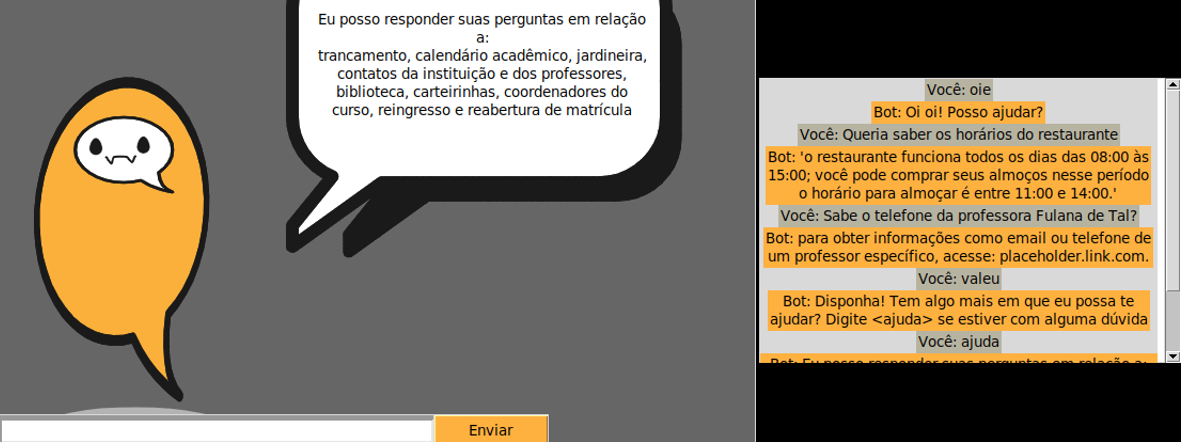
\includegraphics[width=1\textwidth]{fig2.png}
\caption{Interface do {\itshape chatbot} “Kinho”. A interface simples foi escolhida propositalmente para direcionar a atenção dos usuários aos campos textuais. No futuro, uma funcionalidade de voz será integrada ao sistema.}
\label{fig:exampleFig2}
\end{figure}

Cerca de 200 perguntas foram reunidas para a execução dos testes, onde 50 delas possuem erros ortográficos, caracteres especiais, palavras fora do banco de respostas e números. Durante a execução de cada pergunta no {\itshape chatbot} foram verificadas quantas vezes o programa chegou à resposta adequada, em que momentos apenas uma sentença do banco de respostas foi exibida e se um grande número de perguntas consecutivas interferiu no processamento das requisições.

Os testes realizados pelos desenvolvedores chegaram à conclusão que o programa entende e responde corretamente 98\% das perguntas do usuário em linguagem natural contendo uma ou mais palavras-chave correspondentes no banco de respostas. Perguntas consecutivas de diferentes temas não interferem no processamento do programa, desde que a cada interação seja realizada somente uma pergunta com um tema específico.

O {\itshape chatbot} conseguiu efetivamente remover letras maiúsculas e caracteres especiais das perguntas do usuário. Para o banco de dados, o programa conseguiu entender a separação das respostas em 90\% dos testes e exibiu corretamente a sentença na interface com o usuário. Para evitar a exibição de duas respostas distintas em uma mesma interação, algumas respostas contendo caracteres especiais foram colocadas entre aspas simples, separando-as das demais sentenças. Após isso, a exibição de somente uma resposta por pergunta foi 100\% eficiente.

O processamento das perguntas apresenta limitações em relação a erros ortográficos. Se uma palavra é digitada incorretamente, seja por letras dispostas de forma incorreta, números acompanhando a palavra-chave ou mesmo acentuação inadequada, o programa não consegue relacioná-la com palavras similares no banco de dados.

O {\itshape software} também foi disponibilizado para teste para um grupo de 17 estudantes. Para esse teste, uma versão executável do {\itshape chatbot} foi  liberada aos usuários para que eles a executassem no computador sempre que alguma dúvida pertinente surgisse. Ao final do período de testes, os usuários responderam a um questionário avaliativo a respeito da funcionalidade, eficácia, robustez, facilidade e qualidade do {\itshape chatbot}. Após uma análise qualitativa das respostas dos usuários de teste, constatou -se que cerca de 82\% dos estudantes afirmaram que utilizariam o {\itshape chatbot} para obter informações acadêmicas, 75\% afirmaram que o sistema facilita a comunicação do estudante com canais oficiais de comunicação e 89\% observaram a diminuição do tempo de resposta para tirar dúvidas relacionadas à instituição. Uma pergunta também foi levantada sobre se os estudantes em questão utilizariam o sistema nos {\itshape totens} do campus, e 89\% deles responderam que "sim".

\section{Considerações Finais} 

Este artigo apresentou “Kinho”, um {\itshape chatbot} desenvolvido para instituições acadêmicas com intuito de melhorar o acesso à informação por parte dos discentes. Os resultados experimentais mostram que é possível a implementação de um {\itshape chatbot} que auxilie os estudantes a sanarem muitas dúvidas pertinentes em relação ao espaço acadêmico. Os resultados preliminares deixaram claro que os discentes estão abertos a utilização de tal ferramenta.

A implementação de {\itshape chatbots} baseados em NLP apresentam características similares entre si. Seu funcionamento é simples e de fácil desenvolvimento, mas requer recursos adicionais para uma utilização efetiva no espaço acadêmico. Para trabalhos futuros pode ser implementado uma funcionalidade de voz para se comunicar com o usuário, assim como um sistema de aprendizado de máquina para verificar as perguntas que não foram entendidas pelo {\itshape chatbot} e encontrar uma similaridade entre elas, direcionando a melhor resposta para essas perguntas. Também é possível utilizar o Raspberry Pi como servidor {\itshape web}, permitindo o funcionamento de uma página do {\itshape chatbot} na Internet com os mesmos objetivos do projeto apresentado.

\bibliographystyle{sbc}
\bibliography{bibliot}

\end{document}
